\chapter{Nuvem de Conceitos sobre live coding}\label{app:A}

Uma primeira exposição abstrata do \emph{Universo de conceitos} do \emph{live coding} pode ser visualizada na \autoref{fig:nuvemlivecoding}. A figura foi feita com o auxílio de um programa descrito no exemplo A.1. O código-fonte, em linguagem python, foi utilizado para extração parcial do espaço conceitual da pesquisa. 

A biblioteca utilizada, \emph{Wordcloud}, pode ser encontrada em \url{https://github.com/amueller/word_cloud}. 

\begin{figure}[!h]
\begin{center}
\centering
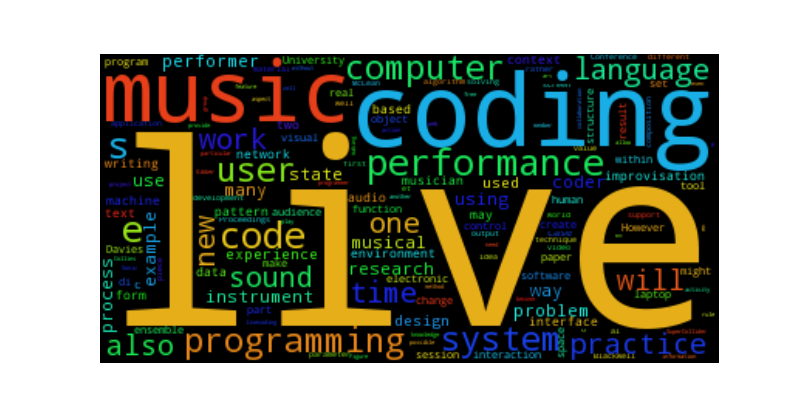
\includegraphics[scale=0.8]{./imagens/livecoding_cloud1.png}
\caption{Nuvem de palavras do \citeonline{ICLC2015},  1$^o$ Congresso Internacional de Live Coding. \textbf{Fonte}: autor.}
\label{fig:nuvemlivecoding}
\end{center}
\end{figure}

O Código abaixo considera a seguinte situação: é possível converter um arquivo de texto em formato \emph{.pdf} para formato \emph{.txt}. Feita a conversão, é possível realizar um levantamento estatístico das palavras mais usadas (o que pode, parcialmente, indicar idéias e conceitos).

 Existem programas online, como o encontrado no link \url{http://convertonlinefree.com/PDFToTXTEN.aspx}, que realizam a conversão. É necessária a correção de alguns erros de caracteres (ver \autoref{fig:utf8}). Além disso, informações de cabeçalho, códigos-fontes, e outros elementos de editoração, foram descartados por considerarmos que não eram parte do corpo textual. Em outras palavras, descartamos palavras que não faziam parte de um discurso de texto, ou atrapalhavam o processo de criação da imagem. O que por sí não resolve todos os problemas, mas auxilia na elaboração da imagem.

\begin{figure}[!h]
  \centering
  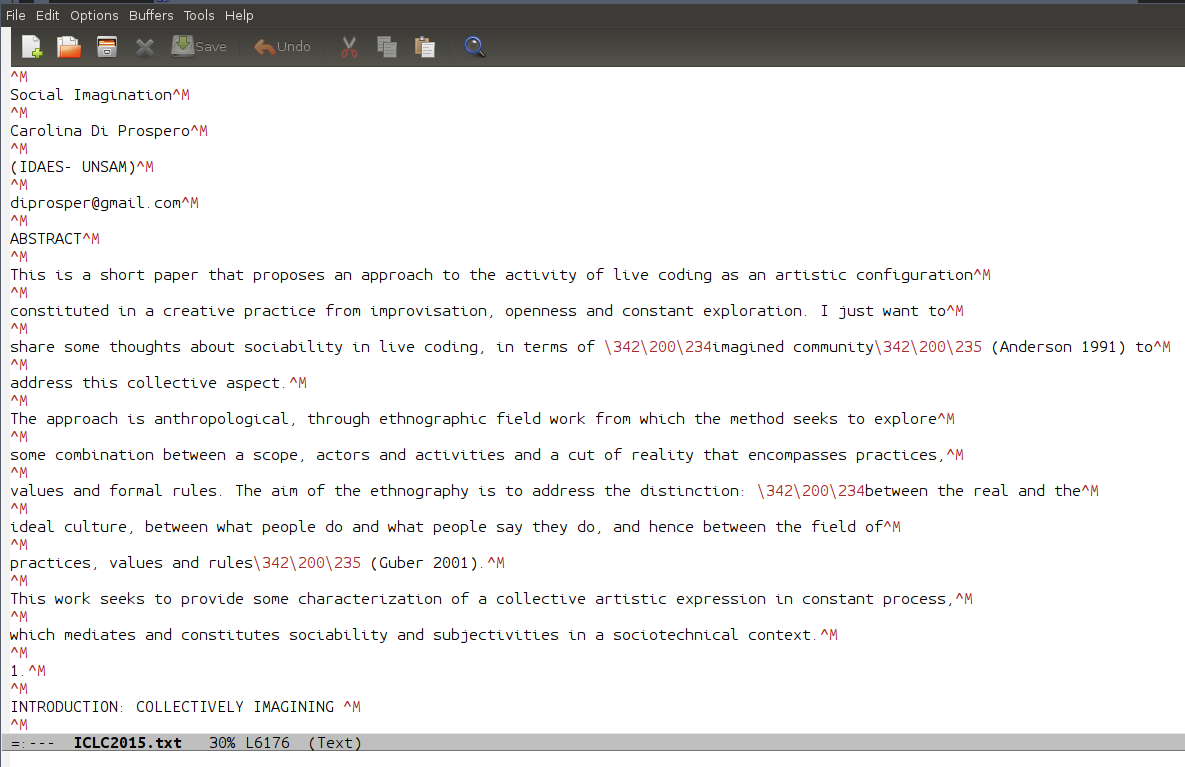
\includegraphics[scale=0.3]{imagens/utf8.png}
  \caption{Resultado da conversão do arquivo \emph{pdf} para \emph{txt} resulta em problemas de codificação que necessitaram ser corrigidos por comparação com o arquivo original. \textbf{Fonte}: autor.}
  \label{fig:utf8}
\end{figure}


\begin{example}{Código-fonte que utiliza a biblioteca wordcloud}  
\begin{minted}{python}
# Bibliotecas utilizadas
from urllib2 import urlopen
from bs4 import *
import re
import datetime
from iso import *
import matplotlib.pyplot as plt
from os import path
from wordcloud import WordCloud
import math
import nltk

from wordcloud import WordCloud
    
# Abra o arquivo em modo de leitura
t = open("ICLC2015.txt", "r").read()

# Gere uma nuvem de palavras
wc = WordCloud().generate(t)
    
# Mostre a imagem gerada com o matplotlib
# levando em conta as frequencias das palavras
plt.figure()
plt.imshow(wc)
plt.axis("off")
plt.show()
\end{minted}
\label{cod:nuvem}
\end{example}

Com auxílio da biblioteca NLTK \disponivelem{http://nltk.org/} , categorizamos a nuvem de conceitos de acordo com sua função textual \ver{cod:nltk}.

\begin{example}{Código-fonte que utiliza a biblioteca wordcloud}  
\begin{minted}{python}
# Abra o arquivo em modo de leitura
t = open("assets/ICLC2015.txt", "r").read()
wc = WordCloud().generate(t)

# Organize as palavras por frequencia
# de presenca no texto
# (defina organiza)
def organiza(t):
  freq = t[1]
  word = t[0]
  g = []
  index = int(math.floor(freq*10))
  if freq >= index/10.0 and freq < (index+1)/10.0:
    print word
    print index
    groups[index-1].append(word)
  return g

# CLASSIFIQUE AS PALAVRAS
def classifica(e):
  return nltk.pos_tag(e)

# Grupo de palavras bi-dimensional
groups = [classifica(grupo) for grupo in [organiza(palavra) for i, palavra in enumerate(wc.words_)]]

# Imprima todos os grupos 
print groups
\end{minted}
\label{cod:nltk}
\end{example}

O código acima gerou uma saída textual que foi reorganizada nas \autoref{tab:nuvem1} e \autoref{tab:nuvem2} Uma breve análise da nuvem de palavras pode elucidar parte de questões-satélites na improvisação de códigos. Filtramos parte dos resultados por conjuntos de funções textuais – sujeitos-humanos, sujeitos-ferramentas (aplicativos), verbos, adjetivos e substantivos – e categorizamos (de 0 a 9) quantas vezes o termo foi utilizado, sendo 0 de 0\% a 10\%, e 90\% a 100\% de uso frequência no texto)

No caso dos sujeitos-humanos, podemos ver nomes de Nick Collins e Alex McLean \ver{sec:tecelagem} e Pietro Grossi \ver{sec:grossi}. No caso dos sujeitos-ferramentas, destacamos o papel do SuperCollider,  do Gibber \cite{roberts_gibber:_2012 2,roberts_web_2013} . Ambos são ambientes de programação para de síntese sonora e composição algorítmica. Uma característica em comum destes ambientes, o procedimento de compilação de códigos, é conhecido como Just In Time \ver{sec:JIT}, dispositivo técnico que permitiu a execução de códigos durante o tempo de execução.

Verbos fornecem informação sobre o comportamento dos improvisadores de códigos. Além da atividades como performatizar e codificar, é notável atividades sociais ligadas à visão, à escrita, à técnica, à lógica. Embora a Música seja a atividade proeminente do live coding, não obtivemos resultados que retornassem, por exemplo, a palavra \emph{hearing}.

Adjetivos destacam características da prática. \emph{Live} é a palavra-chave, e sugere uma prática de performance. Visual sugere uma característica fundamental, tanto quanto a Música, para uma performance. Ensemble destaca a natureza de grupos, isto é, poucas performances solo são realizadas se comparadas às performances de duos, trios. Palavras como university, research e technology, e laptop acusam não apenas uma prática artística, mas um Programa de Investigação Científica. A esfera de pesquisa acadêmica permitiu ramos de desenvolvimento com linguagens de programação, cognição, inteligência artificial, semiologia, performance musical (improvisação), e mais recentemente, antropologia, conferindo à produção de live coding espécie de autenticidade acadêmica.


% http://www.tablesgenerator.com/
\begin{table}[]
\centering
\caption{tab:nuvem1}
\label{my-label}
\resizebox{\textwidth}{!}{%
\begin{tabular}{llllll}
Número Qualitativo/Função & 0 & 1 & 2 & 3 & 4 \\
Pessoas & - & Collins,Blackwell,McLean,Grossi & - & - & - \\
Aplicativos & - & SuperCollider,Gibber,SonicPi & - & - & - \\
Verbos & take, see,shared,networked,explore,made & make, provide,writing,solving, making & used & using,coding & performer \\
Adjetivo ou Numeral, ordinal & less, open,potential,similar,important,cognitive,virtual & first,real,electronic, visual, ensemble,possible, free,livecoding,aspect & musical,many & new, one & - \\
Substantivo & Browser,point,approach,order,node,collaborative,number,source,present,community,server,framework,orchestra,digital,level,kind,type,memory,analysis,line, body,concept,technology,working,org,current,show,mean,end,processes,people,international & University,conference,proceedings,network,interface, environment, text,form, context,musician,space,paper,program, audi-ence, function,change, control,human, laptop,interaction,structure, part,session,tool,result, create,object,case,algorithm,value, develop-ment, material,set, technique,parameter,idea,screen,video, applica-tion, support,composition,piece, knowledge, feature,cell,activity,art,action,information,method,web,rule,group,need,particular,project, allow,collaboration,programmer,member, play,output & use,coder,process,state,example,way,software,research,problem,experience,design,improvi-sation,different,machine,pattern,audio & work,instrument & system,computer,user,language,time,practice,sound
\end{tabular}
}
\end{table}


\begin{table}[]
\centering
\caption{My caption}
\label{my-label}
\begin{tabular}{llllll}
Número Qualitativo/Função & 5 & 6 & 7 & 8 & 9 \\
Pessoas & - & - & - &  &  \\
Aplicativos & - & - & - &  &  \\
Verbos & - & - & - &  &  \\
Adjetivo ou Numeral, ordinal & - & - & - & live &  \\
Substantivo & programming & - & - & performance, code & “livecodecoding”, music
\end{tabular}
\end{table}

